\section{OLED Power Profiling Tools}
\label{sec:tools}

Using the new OLED power model presented in \S\ref{sec:newmodel}, we
have developed two OLED power profiling tools.
%  and an Enhanced Android Battery which provides much more accurate OLED
% power and energy draw estimation than the default Android Battery.

\subsection{Tool 1: Per-Frame OLED Power Profiler}
\label{subsec:analyzer}


% The first tool, a per-frame OLED power  (PFOP) profiler,
\name is a per-frame OLED power profiler designed to enable
an app developer to profile and optimize the OLED power draw of all the
UI components known as views in Android in each app activity design.
The objects in these views fall into two broad categories:
dynamic objects and static objects. Since dynamic objects such as ads or videos
will change in real time, the developer typically focuses on
optimizing the power draw of static objects.
A second design goal of \name is to make it easy-to-use and portable
to any unmodified Android versions.
%  The PFOP analyzr assist the developer to rapidly analyse their apps for
%  display power optimization.

%   Further various views of an App might be designed at different timelines and by different
%   groups. The knowledge of views which are required to be optimized also increases the group
%   productivity, focusing direct effort on these least optimized parts.

%   We observed that Pixel2 and MotoZ3 has a power sensor with
%   sampling rate of approximately 1.4 second. Using this sampling
%   rate the static model generation will take more 12 hrs with 4096
%   piecewise model and more than 1.4 hrs with 512 piecewise model.
%   The main problem here is that we have to take care of the
%   experiment very precisely during the long test duration, i.e. the
%   external environmental conditions like temperature.


%    This happens because the activities are synthetically colored
%    and spread in the histogram happens in case there is a
%    dynamic object which may have continuous textures. When designing
%    the UI, the developer will not consider these objects as these are updated
%    at the runtime.

%   This is also true that designer has to evaluate their app on various devices
%   before they release the app. So modeling and optimising app in various devices is very time
%   consuming and given that UI design consists of a small proportion of colors.

The main challenge of the \name profiler design is to identify all the UI
components of the displayed frame, \eg separating dynamic objects from
static objects, in order to calculate their corresponding OLED power
draw.
% 
% The Challenge is to analyse and determine content of views. Our analysis 
%  determines what are the types of object present on the screen.For example
%  an ImageView or VideoView can be used to determine the dynamic objects.
%  Once the dynamic objects are identified we get it's bounding boxes.
We also need to remove system components on the screen such as the
status bar and the navigational bar.
%  which may also be static.
%   Once all the above mentioned components are removed, the remaining are
%   of the static objects which are for the activity of our interest
%   needing optimisation.


\if 0
There might be some continuous components in the activity which may not contribute
to more than 1\% like the shadowing of the text. For this we switch to the linear model.
As we have seen earlier we estimate the red, blue and green curves in linear RGB,
by only knowing the lowest and highest intensity current. So in total for this we
require 4 more, i.e. red, blue \& green at highest intensity and black
(as for the lowest intensity in all red, green and blue is black) images to evaluate the current.
The error in linear model is high but as it will be a small fraction of the screen,
this error with respect to total display current will be very small.
\fi

\if 0
We generated the histogram of the entire screen. We find all peaks
which have a contribution to more than 1\% of the screen area.  We use
this peaks to generate monochromatic images and generate the current
model for these specific images.  If the peaks doesn't cover 96\% of
the screen we capture an extra of 4 more images (black, red, green and
blue) in the linear model for the remaining of the screen.
\fi

%   For the per component analysis, the most straight forward way is to get
%   the view group of the entire screen and found that this information is
%   not readily available from the system.

The \name profiler breaks down the OLED power draw by a frame in three steps.
First, to identify all the UI
components in a frame, it uses the Android tool ``uiautomator'' to
obtain a dump of the current app screen in xml. {Analyzing the xml
  file gives information about the various views including all the
  system components on the app screen and their bounding boxes.}
Because the system UI components are outside the app view hierarchy,
\name uses the Android command ``dumpsys window windows'' to gather their
bounding boxes.  Second, \name uses the OpenCV library to extract the
pixels within each bounding box.  Finally, it applies the P-LMLR pixel
power model (Eqn.~\ref{eq:first_order_variable}) to derive the OLED power draw for each bounding box and
hence the UI component.


% \paragraph{Implementing the tool as an app.}
To make it easy to use and portable (second design goal),
we implemented \name as an Android
app that only
%   Since an app cannot directly call ``uiautomator'', we created a
%   background running process which calls ``screencap'' to capture
%   the screen shots.  Building the tool
uses built-in tools uiautomator,
dumpsys and screencap.
%   which makes it portable to Android devices with different (unmodified) Android OS versions.
%   In future work, we plan to implement
%   these as system binder \comment{does this require modiying android???}
%   for even lower overhead via piggybacking
%   surface flinger.
\begin{figure}[tp]
	\begin{subfigure}[]{0.30\columnwidth}
		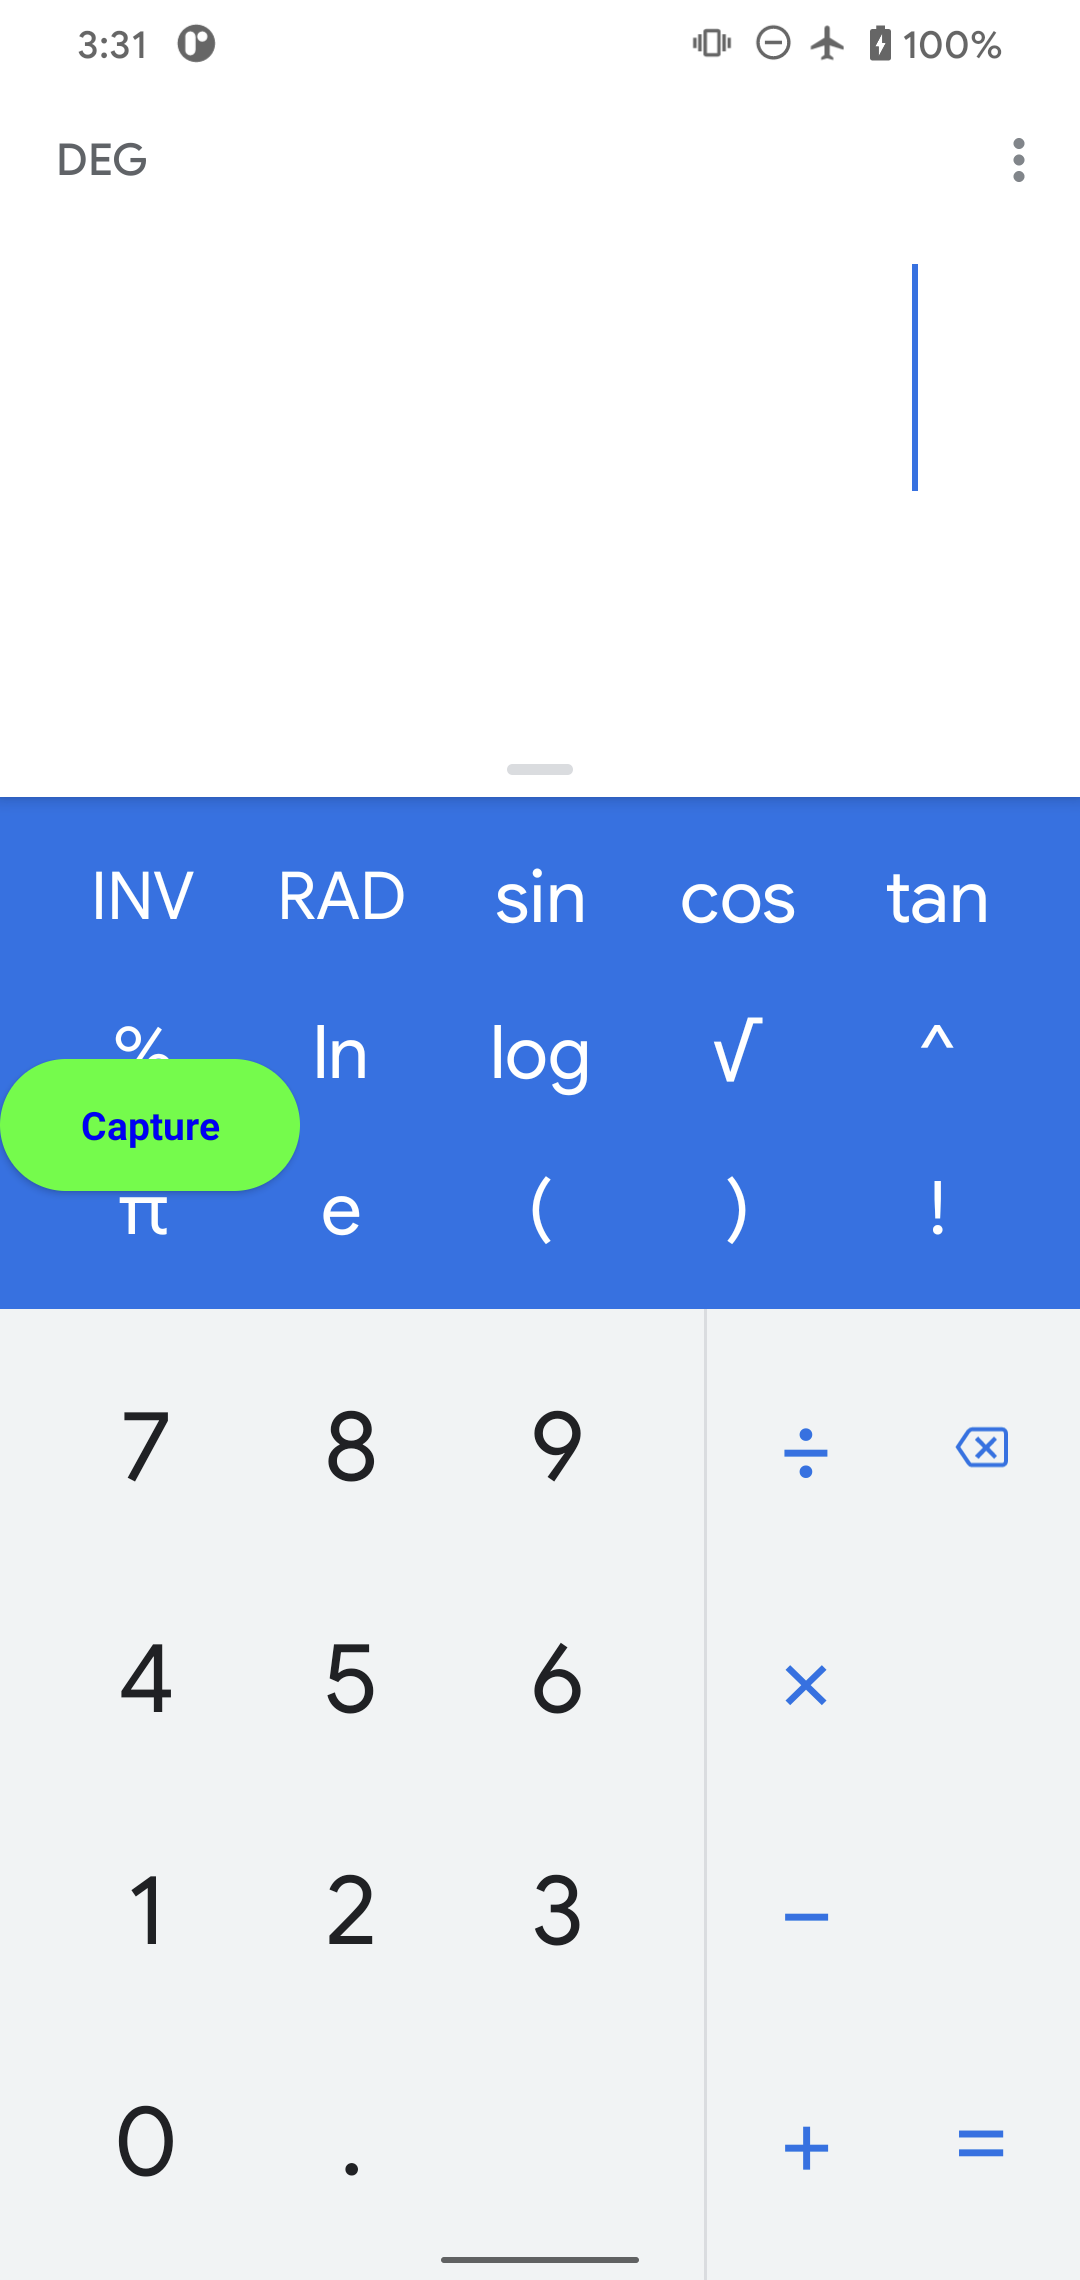
\includegraphics[width=\textwidth]{figure/001_app_capture.png}
		\caption{Floating icon}
		\label{fig:tool1_screenshot_a}
	\end{subfigure}
        \hfill 
%%	\begin{subfigure}[]{0.40\columnwidth}
%%		\includegraphics[width=\textwidth]{./figure/12000b_model.png}
%%		\caption{Show Histogram and option of model}
%%		\label{fig:tool1_screenshot_b}
%%	\end{subfigure}
%%      \\
	\begin{subfigure}[]{0.30\columnwidth}
		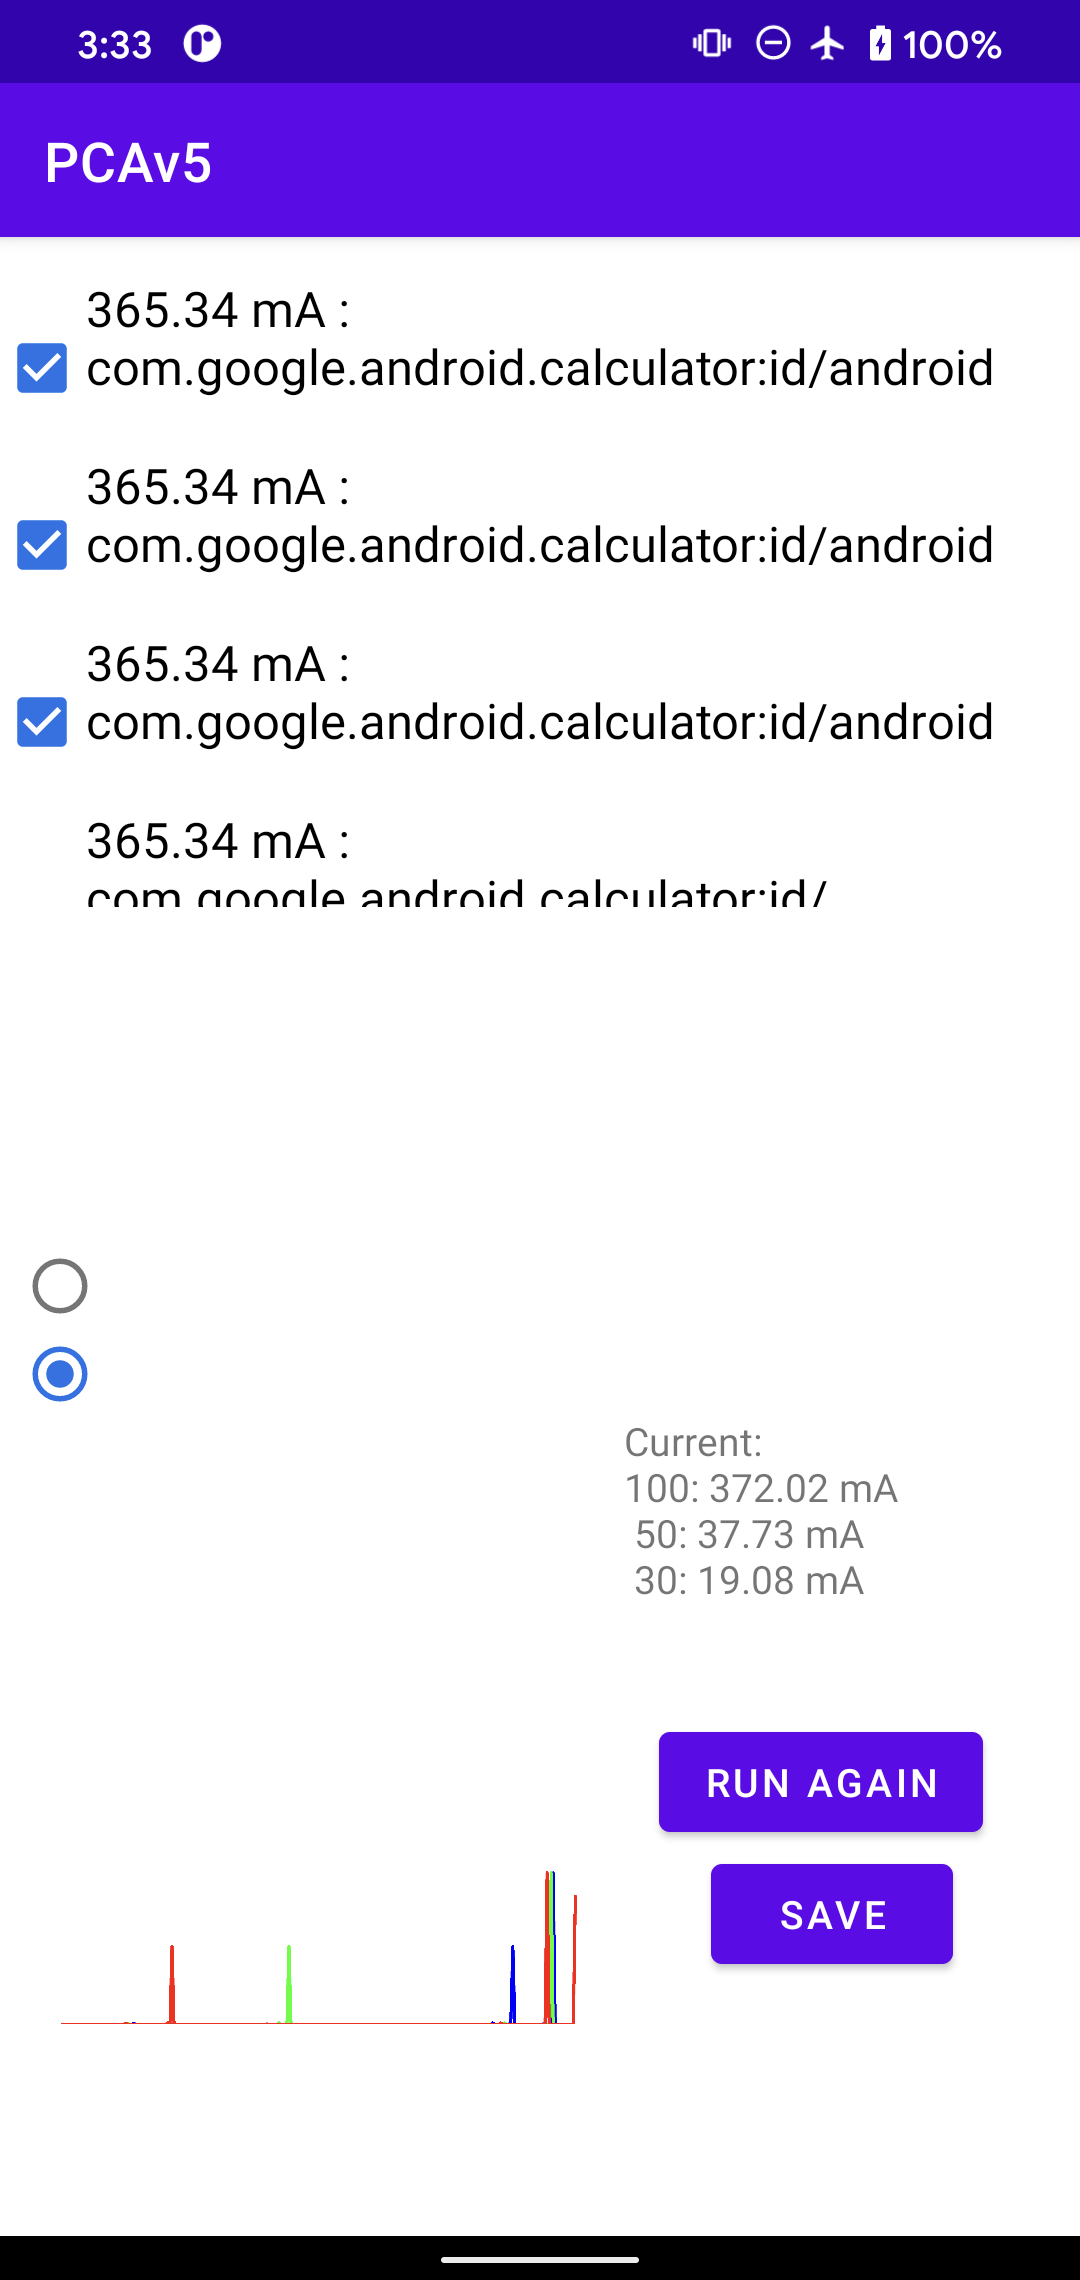
\includegraphics[width=\textwidth]{figure/003_app_histogram.png}
		\caption{Histogram of pixel colors}
		\label{fig:tool1_screenshot_d}
	\end{subfigure}
        \hfill 
	\begin{subfigure}[]{0.30\columnwidth}
		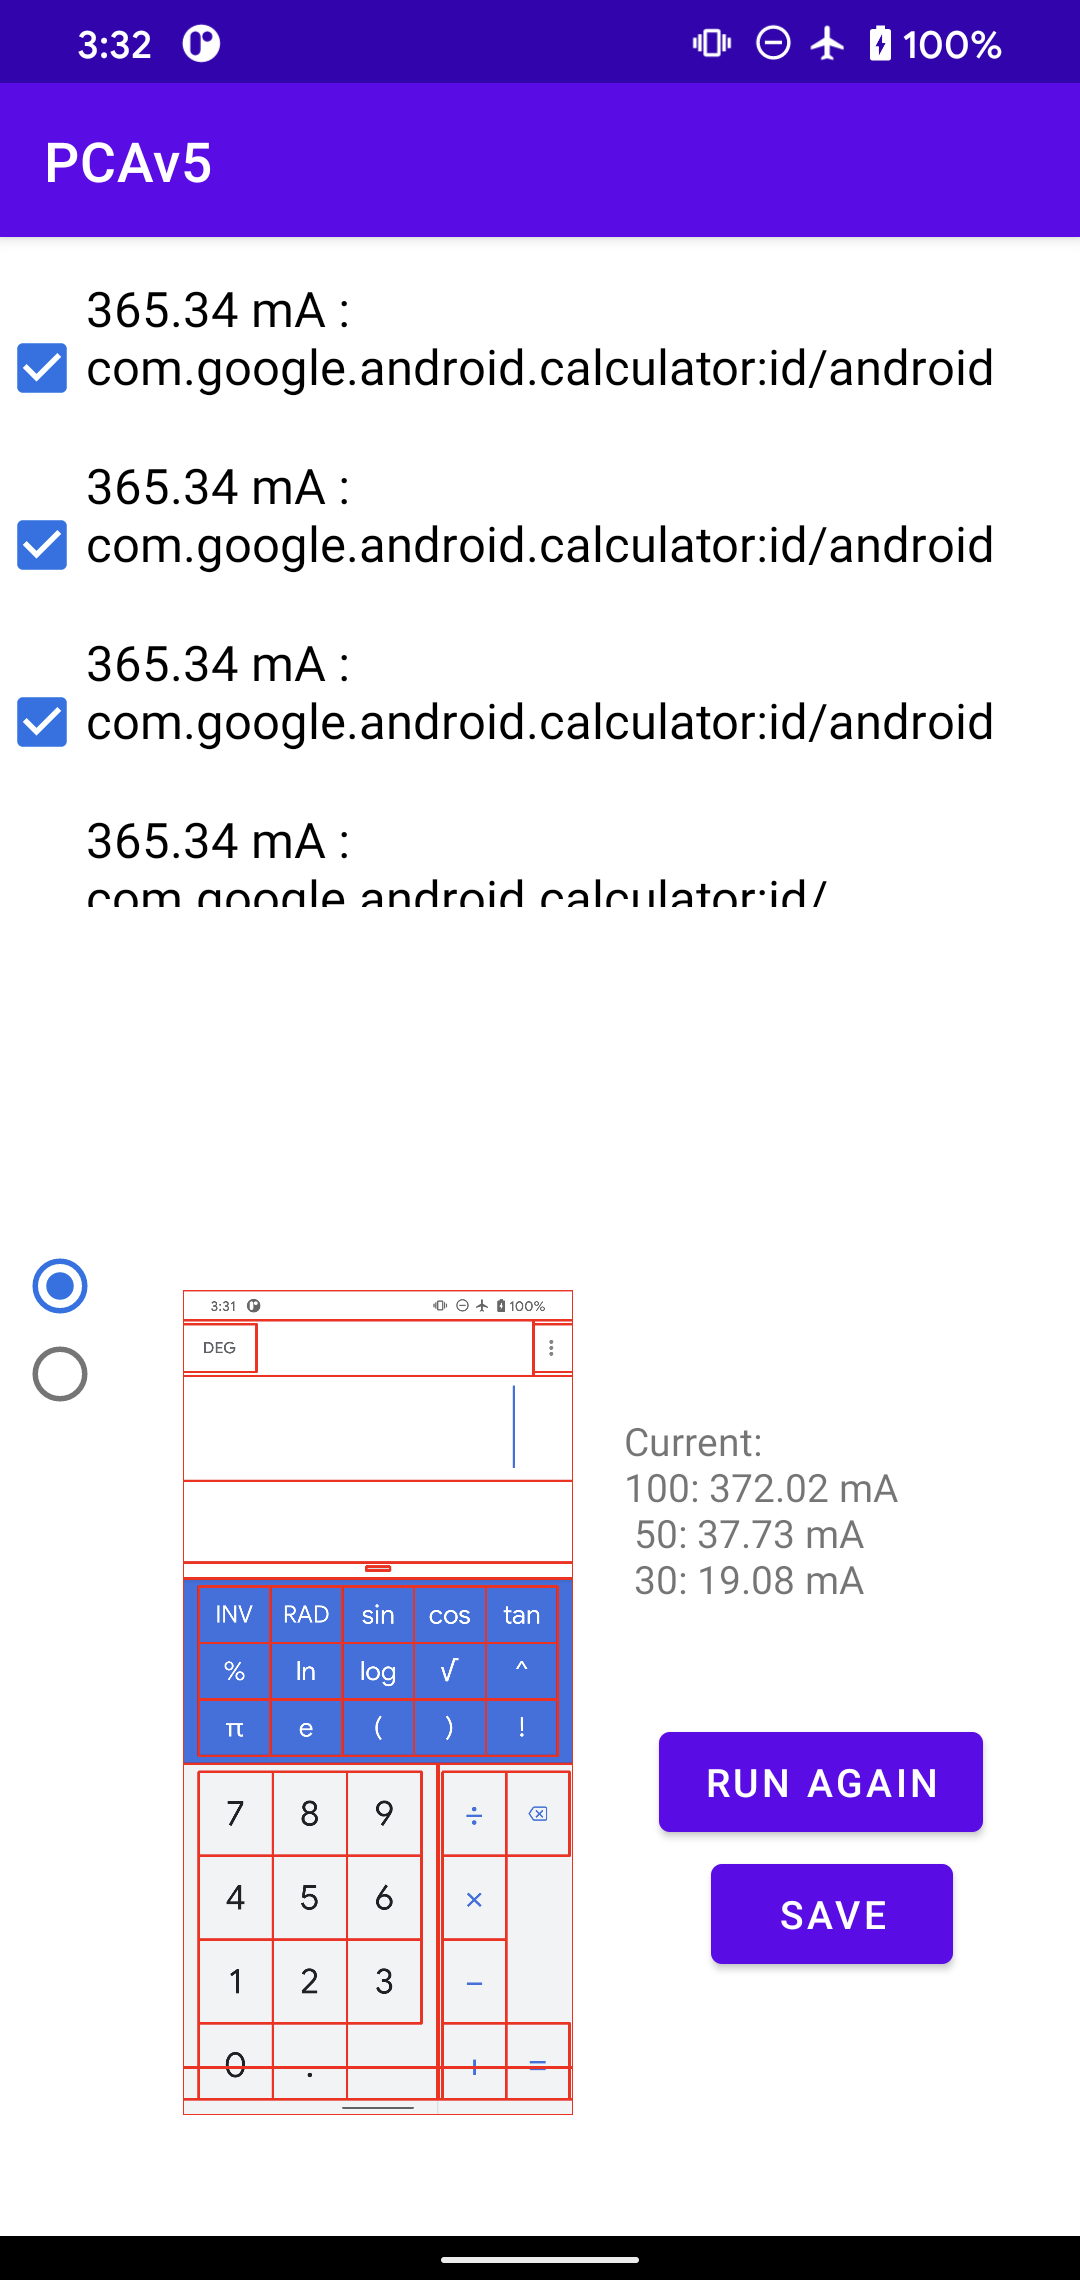
\includegraphics[width=\textwidth]{figure/002_app_break_down.png}
		\caption{Per-UI component current}
		\label{fig:tool1_screenshot_c}
	\end{subfigure}
        \vspace{-0.1in}
	\caption{The \name profiler screen shots on Pixel 4.}
	\label{fig:tool1_screenshot}
    \vspace{-0.2in}
\end{figure}

Figure~\ref{fig:tool1_screenshot} shows the screen shots of the
profiler app in action. The app displays a floating icon which is an Android service
that overlays on top of the app that is running, as shown
in Figure~\ref{fig:tool1_screenshot_a}. Whenever the icon is pressed, it sends
a message to the background process to capture the screen and screen
layout via uiautomator.
\forjnl{The app then prompts a model selection
  activity where the developer can select fast model or pre-generated static model.
  }
% Figure~\ref{fig:tool1_screenshot_b}.  Analysis is shown as
% histogram which shows the color peaks and the time for generating the fast model.
%  The user is given a choice whether to choose fast model or
% the static model.
%   If fast model is selected,
%   the model generation
%   is started, and the user do not have to interact during model
%   generation. Analysis of the Fast model is shown as
For screen analysis, the app can toggle between two outputs.
%  component bounding
% box drawn and the histogram as shown in Figure~\ref{fig:tool1_screenshot_d}.
The first is a histogram showing the number of color peaks in the frame,
% and the time required for fast model generation,
as shown in Figure~\ref{fig:tool1_screenshot_d}.
%   If static model is chosen, is got from the app data.
% Once the model is chosen,
The second is the bounding box of
each selected view and the current per view at 100\%
brightness, as well as the total screen current at 30\%, 50\% and 100\%
brightness, as shown in Figure~\ref{fig:tool1_screenshot_c}.
%  We can chose the components to analyse by selecting the check boxes against them.
%   The app can save the selection,
%   \ie components bounding box and the full screen histogram.
%   We use this tool for our case study.

% We brought the Android screenrecorder and screencap command code. We fetch
% the screen and generate an histogram.
% We identify the peaks. We go into a app training mode where the model is evaluated
% by displaying monochromatic images on the screen. Each of the image is shown for 5 to 10
% seconds.
% If the peaks do not cover 99\% of the screen , we also calibrate 4 more images i.e.
% black, read, green and blue at full intensity for linear model.
% 
% We take the xml file generated by uiautomator to process and generate the bounding boxes
% for every view component.We also identify the type of the views.
% 
% The above display analyser tool is packaged into an android app for ease of use.App provides 
% a per components list for display as output at the end of the analysis.

\begin{table}[tp]
\begin{center}
	\centering
	\caption{\name profiler runtime breakdown (in seconds).}
	\label{tab:tooloverhead}
        \vspace{-0.1in}
    {\footnotesize
%                \begin{tabular*}{\columnwidth}{ | p{0.45\columnwidth} | p{0.12\columnwidth} | p{0.12\columnwidth} | p{0.12\columnwidth} | }
    \begin{tabular}{ | l | c | c | c | }
  	% \begin{tabular*}{\columnwidth}{|l|c|c|c|}
		\hline
		Tool component        	&  Pixel 2 & Moto Z3 & Pixel 4\\
		\hline
		Screen shot	        	&  0.41 & 0.58 & 0.42 \\
		Gathering Bounding box  &  0.38 & 1.08 & 1.84 \\
		Per-UI component current	&  1.47 & 1.32 & 1.84 \\
		Generating Histogram	&  0.14 & 0.15 & 0.17 \\  
		Total frame current     &  0.02 & 0.02 & 0.03 \\
		\hline
	\end{tabular}
	}
\end{center}
\vspace{-0.15in}
\end{table}

\paragraph{Evaluation.}
Since \name is an offline profiler,
we analyze the time it takes to analyze the OLED power draw of a frame.
We break down the time due
to its 5 processing steps: taking a screen shot, gathering the bounding box
data, generating per-UI component current, screen histogram generation,
and calculating the total current for the screen.  The results for the
three phones are shown in Table~\ref{tab:tooloverhead}.  We see that
taking screen shot, gathering bounding boxes, and histogram generation can
take a few seconds. This is the price we pay
for designing \name to be portable, \ie  only using system
commands on unmodified Android versions which do not use sampling.
Nonetheless, the total time for analyzing a frame is less than 4.3
seconds on all three phones.



\if 0
On average the screen shot took for 1.77s for Nexus 6, 617
ms for Pixel 2 and 547ms for Moto Z3.  For gathering bounding box
information, it took on average for 2.56 S for Nexus 6, 1.69 S for
Pixel 2 and 1.54 S for Moto Z3.  The total screen current computation
on an average took 395 mS for Nexus 6, 43 mS for Pixel 2 and 51 mS for
Moto Z3.  Per component current computation depends on the complexity
of the activity. On an average it took for 320 mS for Nexus 6, 132 mS
for Pixel 2 and 147 mS for Moto Z3.  The histogram generation took on
average 3939 mS for Nexus 6, 602 mS for Pixel 2 and 786 mS for Moto
Z3.  After the initial computation the data is stored in memory so
that the toggling between the components selection has very low
overhead.
\fi

\forjnl{Fast modeling depends on the number of peaks in the histogram which
greatly depends on the contents of the screen. On average we observed
that for the chosen app in Table~\ref{tab:activities_peaks} it took
less than 2 minutes on average (8 peak colors for the frame and 4 basic colors
for training the LMLR model).
}

% The screen shot of the output of the app is given in Figure~\ref{fig:tool2_screenshot}.
% \begin{figure}[]
% 	\begin{subfigure}[]{0.4\columnwidth}
% 		\includegraphics[width=\textwidth]{./figure/12000a_per_component_bounding_box.png}
% 		\caption{The app detects the bounding boxes as red of the views.}
% 	\end{subfigure}
% 	\begin{subfigure}[]{0.4\columnwidth}
% 		\includegraphics[width=\textwidth]{./figure/12000b_per_component_list.png}
% 		\caption{The app lists all the per component power.}
% 	\end{subfigure}
%         \vspace{-0.1in}
% 	\caption{Tool 1: Per Component Analyser. \dcomment{Not Complete Yet}}
% 	\label{fig:tool1_screenshot}
% \end{figure}

\if 0
\begin{table}[th]
\begin{center}
	\centering
	\caption{Average number of peaks over activities studied in the popular Google Apps.
		(0.2\% of ratio of 16x16x16 color cube takes 40 to 120 seconds depending of the
		 sampling rate.)}
	\label{tab:activities_peaks}
        \vspace{-0.1in}
	% \begin{tabular*}{\columnwidth}{@{\extracolsep{\fill}}| l | l |}
	\small {
	\begin{tabular*}{\columnwidth}{ | p{0.25\columnwidth} | p{0.14\columnwidth} | p{0.14\columnwidth} | p{0.3\columnwidth} | }
		\hline
		App Name        	&  Dark Mode & Light Mode & Ratio compared to 16x16x16 color cube\\
		\hline
		Calculator		&  3.7 & 3.3 & 0.09 \%\\
		Phone			&  3.1 & 2.5 & 0.08 \%\\
		Google Calender		&  3.6 & 3.5 & 0.09 \%\\
		Google Maps		&  8.3 & 7.8 & 0.20 \%\\  
		News			&  4.7 & 3.3 & 0.11 \%\\
		YouTube			&  6.2 & 5.6 & 0.15 \%\\
		\hline
	\end{tabular*}
	}
\end{center}
\vspace{-0.15in}
\end{table}
\fi
% To evaluate the accuracy of the app we choose various activities listed in Table~\ref{tab:activities_peaks}.


%%%%%%%%%%%%%%%%%%%%%%%%%%%%%%%%%%%%%%%%%%%%%%%%%%%%%%%%%%%%%%%%%%%%%%%%%%%
\input tool2
